\section{Первичная обработка данных}

Весь описываемый процесс происходит в \href{https://github.com/vasalf/hse-web-search-homework/blob/master/1/extract.py}{этом скрипте}.
Скрипт создаёт папку \texttt{extracted} и складывает туда по два файла для каждой страницы: текст и метаинформацию, последняя в формате JSON.
Кроме того, он создаёт отдельный файл для своей первичной статистики и пишет её туда в формате JSON.

\paragraph{Извлечение документов}

Документы лежат в XML-файлах. Для начала, нужно достать их оттуда.

Традиционных подходов к парсингу XML-документов два: DOM и SAX.
Первый проще и мощнее, второй заметно быстрее.
В стандартной библиотеке есть также и третий подход, называемый ElementTree.
Нам не хотелось разбираться с новыми подходами для настолько просто устроенных документов, поэтому мы выбирали между первыми двумя.

Проще всего выбрать DOM, но при этом есть опасность, что целое объектное дерево не поместится в оперативную память.
В таком случае следовало бы выбрать SAX или разобраться с ElementTree/pulldom.

В скрипте эта часть имеет заведённый под неё абстрактный класс — мы специально оставили место под написание SAX-парсера в случае, если самая простая реализация MiniDOM будет слишком ресурсоёмкой.

Эксперимент, однако, показал, что для каждого из десяти документов построенное MiniDOM'ом дерево занимало менее 1.5GiB в оперативной памяти, что при имеющихся у нас вычислительных ресурсах нас более чем устраивало. Соответственно, был оставлен MiniDOM-парсер, как самый простой вариант, не требующий чрезмерных человеческих и вычислительных ресурсов.

После извлечения контента нужно было преобразовать его в строчку. Мы использовали встроенный base64-декодер для получения массива байтов, а дальше перекодировали содержимое из cp1251 в UTF8 через встроенную библиотечку \texttt{codecs}. Причина последнего преобразования в том, что в языке Python гораздо проще работать именно с UTF8-строчками. Да и нам тоже на них приятнее смотреть.

\paragraph{Удаление HTML-разметки}

Мы использовали рекомендованную в тексте задания библиотечку BeautifulSoup.
В документации указан способ прикрутить туда альтернативные парсеры XML. Поскольку реальные данные из интернета вовсе не всегда являются корректными xml-документами, дефолтному парсеру от этих данных стало плохо.
После серии экспериментов мы останосились на \texttt{lxml}, дававшем более чем удовлетворительные результаты.

Из разметки мы извлекли метаинформацию и контент. Метаинформация содержит заголовок страницы, её URL (интересный факт, что не все урлы из коллекции являлись корректными ASCII-строчками), а также список урлов, на которые страница ссылается.

Контент можно доставать из документа, пройдясь по всем текстовым узлам, которые достал BeautifulSoup.
Однако не все узлы подойдут: на страницах есть ещё скрипты и CSS-стили, а также комментарии.
Если скрипты и стили можно отсеять по внешнему тегу, то с комментариями в каком-то смысле вышла беда.
По какой-то причине BeautifulSoup их считает за часть текста, не создавая под них отдельного тега.
Решения, основанные на регулярных выражениях, приводили либо к слишком большому времени обработки страницы, либо не были эффективными и оставляли различные артефакты.
В итоге мы смогли от большинства подобных артефактов избавиться через манипуляцию с параметрами BeautifulSoup, который всё же умеет делать элементы под теги, если правильно его попросить.

\paragraph{Параллелизм}

Обработка гигабайтов данных — непростая задача для питона.
Кроме того, из-за GIL там фактически недоступно многопоточное программирование без выхода в другие языки.
К счастью, первичная обработка идеально параллелится по данным, а значит, использовать многопроцессную архитектуру, по процессу на XML-файл, абсолютно ненакладно.
Мы запускали первичную обработку в 4 процесса и на нашем железе в таком режиме она занимала примерно 18 минут.

\paragraph{Первичная статистика}

Статистика, собранная после первичной обработки, приведена в таблице \ref{primary-stats}.

\begin{table}[h]
\begin{tabular}{|c|c|}
    \hline
        Количество документов                              & 200000 \\
        Средний размер документов в словах                 & 808 \\
        Средний размер документов в байтах                 & 7178 \\
    \hline
\end{tabular}
\caption{Статистика, собранная после первичной обработки}
\label{primary-stats}
\end{table}

Распределение длин документов в словах и в байтах, можно посмотреть на рисунках \ref{primary-length-w} и \ref{primary-length-b}, соотвтетсвенно, а соотношение объёма теста и исходного документа — на рисунке \ref{primary-volfraction}.

\begin{figure}[h]
    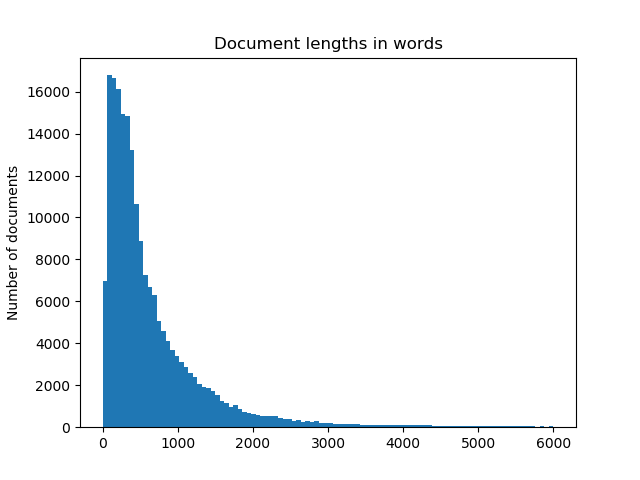
\includegraphics[width=.5\textwidth]{doc_words.png}
\caption{Распределение длин документов в словах}
\label{primary-length-w}
\end{figure}

\begin{figure}[h]
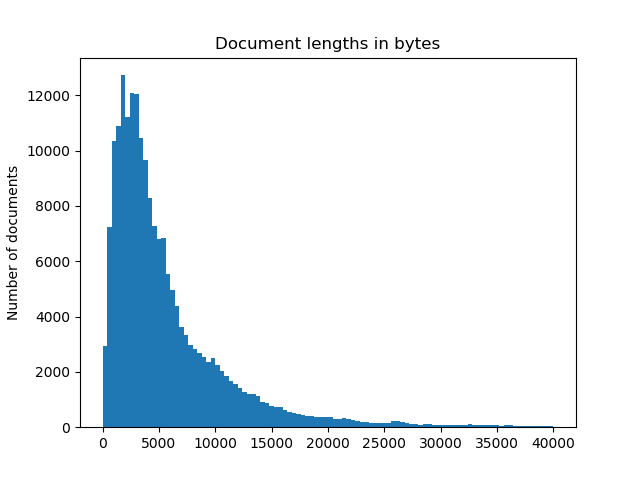
\includegraphics[width=.5\textwidth]{doc_lengths.png}
\caption{Распределение длин документов в байтах}
\label{primary-length-b}
\end{figure}

\begin{figure}[h]
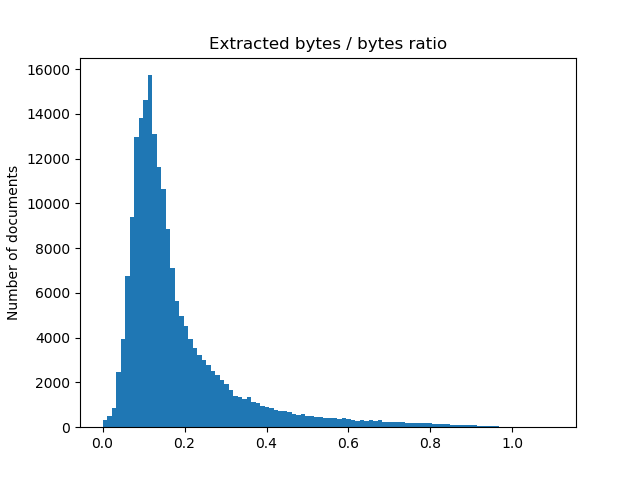
\includegraphics[width=.5\textwidth]{doc_ratio.png}
\caption{Распределение отношения объёмов текста и исходного документа}
\label{primary-volfraction}
\end{figure}
